\documentclass[10pt,a4paper]{article}
\usepackage{amssymb,amsmath}
\usepackage{graphicx,subfigure} 	 
\usepackage{times}
\setlength\parindent{0pt}
\title{UG3 Introduction to Vision and Robotics \\ Vision Assignment}
\author{Clemens Wolff, Toms Bergmanis}
\date{March 7th, 2013}

\begin{document}

\maketitle

\section{Introduction}\label{intro}
Finding (known) objects of interest in an image and following those objects over
a sequence of frames is called object tracking. Its applications are manifold,
ranging from augmented reality to medical imaging.\\
Inter-frame and intra-frame variability make the task a challenging one:
difficulties in tracking can arise due to abrupt object motion, changing 
appearance patterns of both the object and its surroundings, dropped frames,
image noise, and many other factors.\\
This makes general-purpose object tracking a tremendous challenge - and means
that object tracking systems will limit themselves to function under some 
simplifying assumptions and for some specific, well defined task only
\cite{REF}.\\
This report presents an method to track circular red, blue, and green robots 
under varying illumination and scene background conditions. The algorithm is
described in Section \ref{methods} (a sample MATLAB implementation is provided 
as an appendix). Section \ref{results} reports the object tracker's performance
in different capture environments. The results of this evaluation and possible 
avenues for improvement are discussed in Section \ref{discussion}.


\section{Methods}\label{methods}
Several simplifying assumptions were made to constrain the tracking problem.
It was assumed that:
\begin{enumerate}
    \item
    The objects to be tracked will be puck-like "robots", coloured in different
    shades of red, blue, and green.
    \item
    A triangle of a darker colour will sit on top of the robots, indicating
    their directions.
    \item
    The camera observing the scene will be set up in an angle not less than 
    45\% with respect to the plane it is observing. 
    \item
    The background of the scene will have a different colour than the robots.
\end{enumerate}


\subsection{Detection of Robots}\label{coloralgo}
\begin{description}
\item[Input] \hfill \\
    $I$, a three channel image of dimensions $m \times n$ in the RGB colour-space.
\item[Output] \hfill \\
    $M$, a $m \times n \times 3$ binary matrix where for each pixel $P_{ij}$ of
    $I$, it holds that: \\
    $M(i,j,1) = 1 \leftrightarrow P_{ij}$ belongs to the red robot, \\
    $M(i,j,2) = 1 \leftrightarrow P_{ij}$ belongs to the green robot, \\
    $M(i,j,3) = 1 \leftrightarrow P_{ij}$ belongs to the blue robot.
\end{description}
\textbf{Algorithm}
\begin{enumerate}
    \item
    Apply approximate RGB-normalisation to $I$, giving $I_n$:
    \begin{itemize}
        \item
        For each pixel in $I_n$, calculate the sum $S_{rgb}$ of the red, green, 
        and blue values of that pixel.
        \item
        If $S_{rgb} \ne 0$ (the pixel is not absolute black), set each of the 
        pixel's red, green, and blue values to that value divided by $S_{rgb}$.
    \end{itemize}
    \item
    Calculate $\mu_r, \mu_g, \mu_b$ and $\sigma_r, \sigma_g, \sigma_b$, the 
    means and standard deviations of the values in the three channels of $I_n$.
    \item
    Assign each pixel $P_{ij}$ in $I$ to one of the robots or to the background:
    \begin{itemize}
        \item
        Normalise $P$'s red, green, and blue values, giving $P_n$.
        \item
        Calculate the probabilities $p_r, p_g, p_b$ that $P_n$ was generated 
        by the Gaussian distributions $\mathcal{N}_r = (\mu_r, \sigma_r),
        \mathcal{N}_g = (\mu_g, \sigma_g), \mathcal{N}_b = (\mu_b, \sigma_b)$.
        \item
        Calculate $P$'s hue value $h$.
        \item
        If $h$ is within a certain range defined as red and $p_r$ is
        sufficiently small, set $M(i,j,1) = 1$ (similarly for ranges defined as
        green/blue and $p_g$/$p_b$. If none of these conditions are met, set
        $M(i,j,1) = M(i,j,2) = M(i,j,3) = 0$.
    \end{itemize}
    \item
    Remove noise from each channel in $M$:
    \begin{itemize}
        \item
        Set pixels to zero if they have fewer neighbours with value one than
        they have adjacent pixels with value zero.
        \item
        Set zero-valued pixels to one if they have two one-valued 
        horizontal or vertical neighbours.
    \end{itemize}
    \item
    Remove components that are distant from the main concentration of mass in
    each channel in $M$:
    \begin{itemize}
        \item
        Compute the centre of mass $C$ of the channel.
        \item
        Compute $c_1, c_2, \ldots$, the centres of mass of each connected 
        component in the channel.
        \item
        Compute the mean distance $\delta$ of the $c_k$ to $C$.
        \item
        Set $M(i,j) = 0$ for all the pixels $(i,j)$ in the components $k$ that
        satisfy $c_k > \tau \delta$ for some fixed threshold $\tau$.
    \end{itemize}
    \item
    Exploit the fact that all robots have similar sizes by setting every channel
    in $M$ to all-zeros if the number of pixels set in that channel is smaller
    than the number of pixels set in the most populated channel by some margin.
\end{enumerate} 
\begin{figure}[ht]
    \centering
    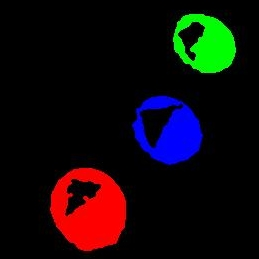
\includegraphics[width=40mm]{src/d1_i5_blob_mask.jpg}
    \caption{Result of Robot detection}
    \label{colorfig}
\end{figure} 
Figure \ref{colorfig} shows a visualisation of the output matrix $M$.

\subsection{Finding Robot Directions}\label{directionalgo}
\begin{description}
\item[Input] \hfill \\
    $I$, a three channel image of dimensions $m \times n$ in the RGB colour-space.
\item[Output] \hfill \\
    $\Lambda = \{(c^m_r, c^t_r), (c^m_g, c^t_g), (c^m_b, c^t_b)\}$, a set where
    $c^m_r$ is the centre of mass of the red robot and $c^t_r$ is the point 
    towards which the robot is facing (similarly for the green and blue robots).
\end{description}
\textbf{Algorithm}
\begin{enumerate}
    \item
    Get a matrix of robot masks $M$ using the algorithm in Section 
    \ref{coloralgo}. Let $M_i$ be the i$^{th}$ channel of $M$ i.e. the set of
    points $\{M(a,b,i) | 1 \le a \le m, 1 \le b \le n\}$.\\
    Apply the remainder of the algorithm to each channel $\xi$ in $M$.
    \item
    Calculate the convex hull $H$ of the points in the channel and create the 
    set of pixels of $I$ that are inside $H$: $P = \{p_{ij} | p_{ij} \in \xi 
    \land M(i,j,\xi) = 1\}$
    \item
    Calculate $\mu$, the average rgb-value over $P$. Generate 
    $\Pi = \{p | p \in P \land rgbvalue(p) < \mu\}$, the set of pixels in $P$ 
    that have a below-average rgb value.
    \item
    The black triangles on the robots are the pixels in $\Pi$. Get rid of them
    by setting the relevant indices in $M$ to zero.\\
    Recompute the convex hull of $M$.
    \begin{figure}[ht]
        \begin{center}
            \subfigure[After Removing Triangles]{
                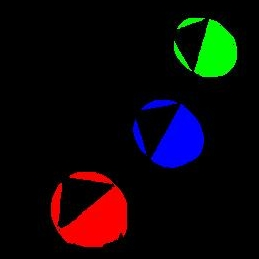
\includegraphics[width=40mm]{src/d1_i5_demasked_triangles.jpg}}
            \subfigure[Removed Triangles]{
                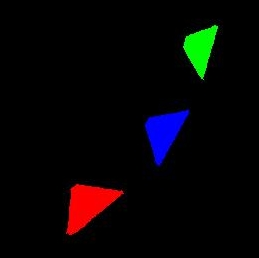
\includegraphics[width=40mm]{src/d1_i5_triangles.jpg}}
        \end{center}
        \caption{Triangle Detection via Local Thresholding}
        \label{trianglefig}
    \end{figure} 
    \item
    Repeat the previous step and remember the pixels in $\Pi$. \\
    This reduces noise in $M$ by giving a tighter estimate on the robot's
    pixels when the triangles were under-detected by the algorithm in 
    Section \ref{coloralgo}. \\
    Figure \ref{trianglefig} shows the result of this step - a notable
    improvement in clarity of the triangles compared to Figure \ref{colorfig}.
    \item
    Update $\Lambda$: $c^m_\xi$ is the centre of mass of $M_\xi$, $c^t_\xi$ is 
    the centre of mass of $\Pi$. \\
    A line from $c^m_\xi$ to $c^t_\xi$ indicates the direction of the robot.
\end{enumerate} 
\begin{figure}[ht]
    \centering
    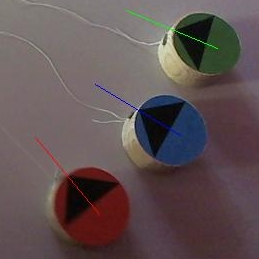
\includegraphics[width=40mm]{src/d1_i5_result.jpg}
    \caption{Detected Directions}
    \label{directionfig}
\end{figure} 
Figure \ref{directionfig} shows a visualisation of the output set $\Lambda$.

\subsection{Tracking Robots Over a Sequences of Frames}\label{trackingalgo}
\begin{description}
\item[Input] \hfill \\
    $\Upsilon = \{I_1, I_2, \cdots\}$, a sequence where each of the $I_i$ is a 
    three channel image of dimensions $m \times n$ in the RGB colour-space.
\item[Output] \hfill \\
    $\Omega$, a visualisation of the robot positions over $\Upsilon$.
\end{description}
\textbf{Algorithm}
\begin{enumerate}
    \item
    Use a median-filter to generate a background $\Omega$ from $\Upsilon$. \\
    For each $1 \le i \le m, 1 \le j \le n$:
    \begin{itemize}
        \item
        Create $\omega_{ij} = \{I_k(i,j) | I_k \in \Upsilon\}$, the set of the 
        colours of the pixels at location $(i,j)$ of all the images in 
        $\Upsilon$.
        \item
        Set $\Omega(i,j) = median(\omega_{ij})$.
    \end{itemize}
    \item
    For each $I_i \in \Upsilon$:
    \begin{itemize}
        \item
        Use the algorithm in Section \ref{directionalgo} to get the set 
        $\Lambda$. Let $\lambda = \{c | (c, \_) \in \Lambda\}$.
        \item
        Overlay $\Omega$ with a line from each element in $\lambda_{i-1}$ to 
        the corresponding element in $\lambda_i$, thus linking the centroids 
        from image $I_{i-1}$ to the centroids in image $I_i$.
    \end{itemize}
\end{enumerate} 
Figure \ref{trackingfig} shows a visualisation of the resulting track.
\begin{figure}[ht]
    \begin{center}
    \subfigure[Data-set 1]{
        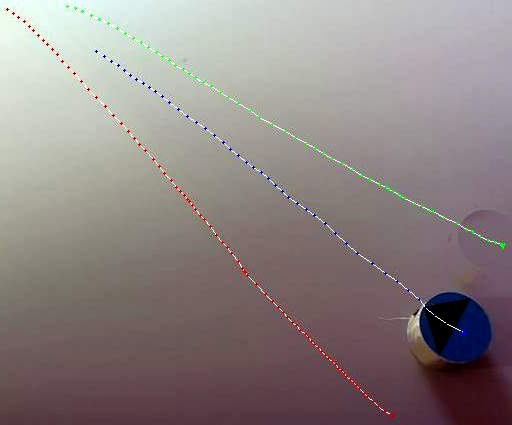
\includegraphics[height=40mm]{src/d1_trace.jpg}}
    \subfigure[Data-set 2]{
        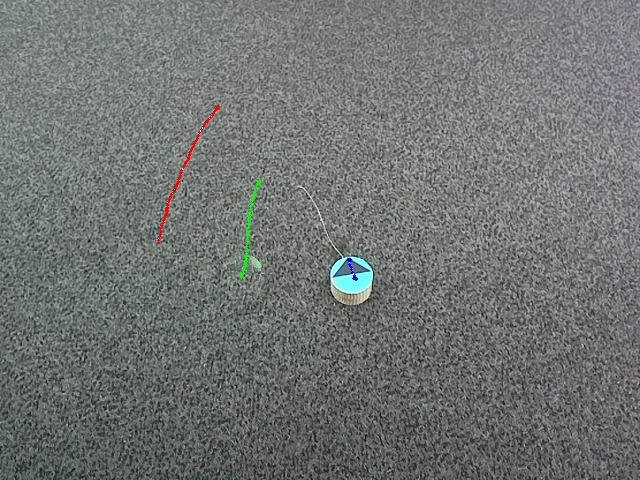
\includegraphics[height=40mm]{src/d2_trace.jpg}}
    \end{center}
    \caption{Output of Tracing Algorithm}
    \label{trackingfig}
\end{figure}


\section{Results}\label{results}
This section evaluates and visualises the performance of the three algorithms 
presented in Sections \ref{coloralgo}, \ref{directionalgo}, and 
\ref{trackingalgo}. Table \ref{datasetpropstable} describes the properties of 
the data-sets used for this evaluation.
\begin{table}[ht]
\begin{tabular}{|l || l | l | p{2cm} | p{4cm}|}
\hline
\# & Background & Robot Size & Robot Colour & Illumination \\
\hline
1 & uniform, grey & large & saturated, dark & uniform, red hue \\
\hline
2 & noisy, grey & small & faded, blue robot is cyan & 
    histograms are bell-shaped \\
\hline
3 & patterned, brown & large & saturated & daylight only \\
\hline
4 & patterned, brown & large & saturated & daylight and artificial 
    light \\
\hline
\end{tabular}
\caption{Properties of evaluation data-sets}
\label{datasetpropstable}
\end{table}

\subsection{Detection of Robots}\label{colorresults}
The algorithm described in Section \ref{coloralgo}, worked perfectly on 
data-sets 1 and 2.
Evaluation on the third data-set led to the worst performance over all data-sets, 
with $\sim$60\% of the occurrences of the blue robot being undetected and 
$\sim$40\% of the occurrences of the green robot being under-detected (leading 
to bad direction detection).
The performance on the fourth data-set was interesting: the red robot was under-
detected in $\sim$45\% of the cases (with the blue and green robots being
found just fine) - while in the other data-sets the red robot was usually
detected with the highest confidence.
Over all four data-sets, about 10\% of the robot instances were badly detected.\\
The fact that the colour-detection algorithm works well on both data-sets 1 and 2
leads to the conjecture that it is invariant under texture changes in the scene 
background and variations in robot-colour saturation.
The bad performance on data-set 3 can be explained by interference from the colour
of the scene background and by changes in scene illumination. The fact that the
algorithm offers almost top-level performance on data-set 4 (captured on the same
background as data-set 3) implies that the change in scene illumination is
probably the largest influence on the algorithm's performance.\\
This is in keeping with the intuition that daylight has more inherent variation
than artificial light, thus introducing a higher degree of variability into the
characteristics of the captured images.

\subsection{Detection of Directions}\label{directionresults}
Performance of robot direction detection, understandably, is heavily dependent 
on the performance of the detection of the robots. If the robots are well
isolated by Section \ref{coloralgo}'s algorithm, robot orientations are 
perfectly detected.\\
The algorithm is invariant under loose detection - false positive cases where 
some addition non-robot region is misleadingly detected as a robot. This is 
due to the algorithm's ability to filter-out noisy detections.\\
In case of under-detection - false negative cases where some parts of the image
representing the robot where not detected - the algorithm breaks: the predicted
direction is skewed towards the opposite side of the under-detection. This is
due to the algorithm not putting strict circular or ellipsoidal constraints on 
the shape of the robots: under detection is thus able to move the centre of 
mass of either the triangle or the robot-convex-hull. The error introduced by 
this is proportional to the area of the under-detected region.
\begin{figure}[ht]
    \begin{center}
        \subfigure[Loose hull detection]{
            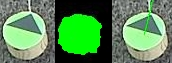
\includegraphics[width=40mm]{src/d2_i32_loose_detection_example.jpg}}
        \subfigure[Hull under detection]{
            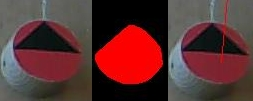
\includegraphics[width=40mm]{src/d4_i66_bad_detection_example.jpg}}
        \subfigure[Good hull detection]{
            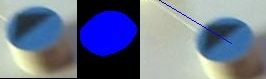
\includegraphics[width=40mm]{src/d1_i100_good_detection_example.jpg}}
    \end{center}
    \caption{Direction detections for convex hulls of different qualities}
\end{figure} 

\subsection{Tracking of the robots}\label{trackingresults}
Section \ref{trackingalgo}'s algorithm to track robots over consecutive frames
is trivial - a mere visualisation of half of the results of the robot-direction-
detection algorithm presented in Section \ref{directionalgo}. The tracking 
algorithm's performance is therefore directly related to the performance of 
the robot-direction-detection algorithm and the same observations as in Section
\ref{directionresults} apply: generally speaking, the algorithm performed 
well.\\
Figure \ref{trackingfig} begets one additional observation related to the
evaluation of the robot-tracking algorithm: both data-sets considered in this
report exhibit the property that one of the objects of interest does not move
much for most of the frames. This entails that generating a background from
data employing a simple frame-difference base approach (such as the median-
filter used in Section \ref{trackingalgo}) to perform background subtraction 
is bound to  fail as one of the objects of interest will be considered a part 
of the background due to being mostly stationary. This is unfortunate since
pre-processing the data-sets with background subtraction would increase the
accuracy of Section \ref{coloralgo}'s algorithm by reducing noise and increasing
resolution in the image.


\section{Discussion}\label{discussion}
The algorithms in Sections \ref{coloralgo}, \ref{directionalgo}, and 
\ref{trackingalgo} operate under a limited number of reasonable simplifying
assumptions and performed well across a range of data-sets captured under very
different conditions.\\
The robot colour detection algorithm of Section \ref{coloralgo} could be improved
by adding more stringent conditions on the shape of the robots e.g. fitting a
circle or ellipse to them rather than a convex hull. This should improve the
subsequent performance of the direction-detection algorithm by reducing the
amount of under-detections.\\
If assumptions about the size, scale, and shape of the robots can be made, Hugh 
transforms or other shape-based techniques could be used to detect the robots.
This would be more robust than the current colour/pixel based approach but not 
invariant under scale or differences in camera positions.\\
Another way to improve the detection of the robots could be augmenting the
current approach with the utilisation of second order spatial image statistics
to pre-process the images. This would lead to a rough estimate of the robot
positions with few false negatives, thus improving the currently utilised
algorithms due to a reduced search space (implying a denser signal). A reduced
search space also allows for computationally expensive but high-precision 
techniques to be used. One example of such a technique is a local colour-based
search starting from a small seed of pixels that are hypothesised to be part of
a robot.\\
Direction detection could be improved by making it less dependent on the
accuracy of the robot detection. One way to achieve this would be to base the 
direction calculation on properties of the detected triangles (e.g. direction =
tangent line to the longest side) rather than on the triangles' centres of 
mass. This would increase robustness to under-detections.\\
Cross-frame tracking could be improved by abusing spatio-temporal proximity. One
way to do this would be put a cap on how far the centroid of the robot can move 
in a certain frame interval, thus smoothing out the odd completely wrong 
prediction.

\bibliographystyle{IEEEtran}
\begin{thebibliography}{10}
\bibitem{REF} Yilmaz, A., Javed, O., and Shah, M., 
``Object Tracking: A Survey'', 
ACM Comput. Surv. 38, 4, Article 13, 2006.  
\end{thebibliography}
\end{document}
